\section{Evaluation on Real Data}
\label{sec:realdata}

All analyses use public data; only aggregate results are reported. Code and result files are in the repository (Section~\ref{sec:statements}).

\subsection{DROZY}
\label{sec:drozy}
\paragraph*{Data} DROZY~\cite{massoz2016ulg} contains 14 adults who each performed three 10-min PVTs while staying awake from the morning of the first test to the third: at about 10:00 (rested), about 03:40 the next night and about 12:00 the next day, rating the KSS at each test. For each test it provides the PVT responses, near-infrared face video from a Kinect sensor, 68 facial landmarks per frame and the vertical electro-oculogram (EOG). Five tests are missing and one did not take place, leaving 36 tests (12 per test number). Video was recorded at about 30 frames per second in all 12 first tests but at about 15 in 8 of the 12 second and 8 of the 12 third tests, so frame rate is confounded with sleep deprivation. Mean KSS rose from 3.25 to 5.58 to 7.33 across the tests.

\paragraph*{Signals and sleepiness} Using the eye aspect ratio from the landmarks~\cite{soukupova2016real} as the closure score, the website's blink meter gave per-test features whose within-person (repeated-measures~\cite{bakdash2017repeated}) correlations with KSS were 0.77 for PVT median reaction time, 0.73 for lapses, 0.53 for PERCLOS, 0.51 for blink duration and 0.35 (not significant) for blink rate (21 degrees of freedom, 13 subjects). Because KSS and every feature also rise with test number, these correlations include the shared time course. The within-person forward-model slopes (Table~\ref{tab:params}) were 18.85~ms of median reaction time, 11.1~ms of blink duration and 0.62 percentage points of PERCLOS per KSS point. The lag-1 autocorrelation of successive minutes was 0.32 for PERCLOS and 0.02 for blink duration, which set $\kappa$.

\paragraph*{Blink counting against EOG} As a reference we detected blinks in the vertical EOG automatically (band-pass 0.5--15~Hz, prominence at least five scaled median absolute deviations, width 40--600~ms); events were not annotated by hand. Across the 36 tests, the meter's blink rates from the landmarks agreed with EOG blink rates (Spearman $\rho = 0.88$; Pearson $r = 0.89$), with a mean difference of $-5.4$ blinks~min$^{-1}$ and 95\% limits of agreement~\cite{bland1986statistical} from $-19.1$ to $+8.3$.

\subsection{The webcam pipeline on DROZY video}
\label{sec:mediapipe}
The comparison above tests the blink logic on landmark data, not the pipeline the website runs. We therefore ran the website's MediaPipe model file on every frame of the 36 DROZY videos and passed the mean \texttt{eyeBlink} score through the unchanged blink meter (Fig.~\ref{fig:mediapipe}). A face was found in 99.9\% of frames (minimum 98.1\% in any test).

Blink rates from this pipeline agreed with EOG blink rates across tests (Spearman $\rho = 0.71$) and within person ($r = 0.65$, $p < 0.001$), but undercounted them by 13.0 blinks~min$^{-1}$ on average (limits of agreement $-35.8$ to $+9.8$). Mean blink duration agreed with the landmark pipeline ($\rho = 0.72$) and rose with KSS within person ($r = 0.58$, $p = 0.004$), as did the number of long closures per minute ($r = 0.51$, $p = 0.013$).

PERCLOS failed. In these near-infrared videos MediaPipe's closure score peaked at 0.68 on average (99th percentile per test; maximum 0.79), so the normalised closure rarely reached the 0.8 PERCLOS level and PERCLOS was below 0.5\% in all 36 tests; it was not related to KSS ($r = 0.22$, $p = 0.32$). When each test's raw score was instead rescaled between its own 5th and 99.5th percentiles, a diagnostic that needs the whole recording, PERCLOS agreed with the landmark PERCLOS ($\rho = 0.86$) and rose with KSS within person ($r = 0.58$, $p = 0.004$), and blink-rate agreement with EOG improved to $\rho = 0.82$. The released model therefore ignores PERCLOS when the camera's blinks do not reach full closure (Section~\ref{sec:system}); an online version of the rescaling is implemented for future validation but is not used. The lag-1 autocorrelation of MediaPipe blink duration was 0.39, against 0.05 for the landmark pipeline, so the released $\kappa$ for blink duration is likely too small for the website's pipeline. Restricting to the 20 tests recorded at 30 frames per second gave similar agreement with EOG ($\rho = 0.83$).

\begin{figure*}[t]
  \centering
  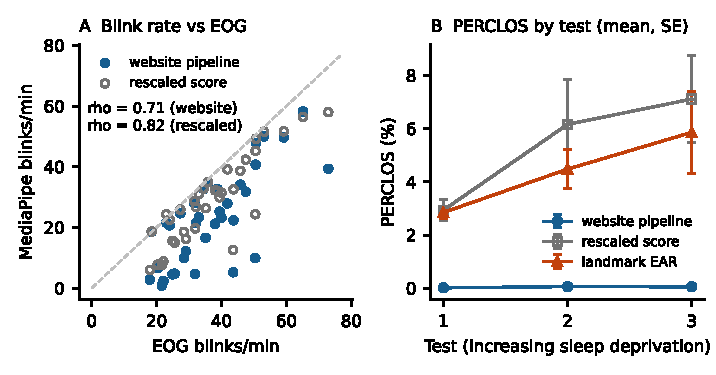
\includegraphics[width=\textwidth]{fig_drozy_mediapipe.pdf}
  \caption{The website's webcam pipeline (MediaPipe \texttt{eyeBlink} blendshapes and the unchanged blink meter) run on the 36 DROZY near-infrared videos. (A)~Blink rate against EOG blink rate, for the website pipeline and for a diagnostic per-test rescaling of the raw score. (B)~Mean PERCLOS by test (SE): the website pipeline stays near zero because the raw score rarely approaches 1. (C)~Mean blink duration from the website pipeline against KSS, one line per subject.}
  \label{fig:mediapipe}
\end{figure*}

\subsection{Replay of the released model on DROZY}
\label{sec:replay}
\paragraph*{Design} For each subject in turn, the forward models were refitted on the other 13 subjects. The model then replayed that subject's real test times, PVT median reaction times and per-minute webcam features (from the landmark pipeline), with or without the KSS rating of the first test as a check-in, and predicted the KSS of each later test from the events before it. DROZY does not record wake time, so we assumed waking at 07:00 after 7.5~h on the day of the first test, with 06:00 and 08:00 as sensitivity analyses. Each rating was placed 11~min after the start of its test. Confidence intervals come from 2000 bootstrap resamples of subjects. Conditions with a check-in need the first test, so they have 20 predictions from 10 subjects, against 24 from 12 subjects without.

\paragraph*{Results} The mean absolute error (MAE) was 1.73 KSS points for the prior alone, 1.51 for the PVT alone, 1.47 for the PVT and webcam, 1.51 for the check-in alone, 1.46 for the check-in and PVT, and 1.38 for all three (Fig.~\ref{fig:replay}). The prior over-predicted sleepiness on average (mean error $+0.81$), mostly at the night test (MAE 2.27 at test~2 against 1.18 at test~3); with all sources the mean error fell to $+0.31$ and the test-2 MAE to 1.60. Results were stable to the assumed wake time (all sources: 1.39 at 06:00 and 1.37 at 08:00; prior: 1.75 and 1.71). With two check-ins, predicting the third test (9 subjects), check-ins alone gave 1.90 and all sources 1.78; both under-predicted the final rating.

These results are indicative only. The intervals overlap widely, conditions with and without a check-in differ in their predictions, and two naive baselines bracket the model: carrying the first rating forward gave 3.45, but predicting each test by the mean rating of that test in the other subjects gave 1.39. That baseline knows the protocol, which a person's daily life does not provide, but it shows that the prior's time course, in particular its night-time level, is the largest source of error here.

\begin{figure}[t]
  \centering
  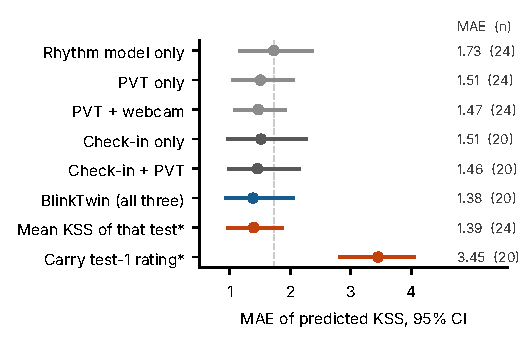
\includegraphics[width=\columnwidth]{fig_drozy_twin.pdf}
  \caption{Leave-one-subject-out replay of the released model on DROZY: MAE of predicted KSS for tests 2 and 3 (95\% CI over subjects; n = predictions). The check-in is the rating at test~1. *Naive baselines; the first uses the protocol's average course.}
  \label{fig:replay}
\end{figure}

\subsection{OpenNeuro ds004902}
\label{sec:openneuro}
\paragraph*{Data} The dataset contains 71 adults tested once after normal sleep and once after a night of sleep deprivation, in counterbalanced order~\cite{xiang2024resting,xiang2024ds004902}. We used only the participant table (version 1.0.4). KSS and SSS were collected in different participants, and only 2 people have both KSS and PVT data in both sessions.

\paragraph*{Group effects and a labelling discrepancy} After sleep deprivation, KSS rose by 2.03 points ($n = 33$, $d_z = 1.00$), the SSS by 1.66 ($n = 35$, $d_z = 0.80$) and the PVT median reaction time by 41.2~ms ($n = 30$, $d_z = 1.33$), while the number of lapses did not change ($p = 0.92$). KSS rose in 73\% of people, stayed the same in 18\% and fell in 9\%. Our paired $t$ statistics for the three PVT columns ($0.04$, $7.31$ and $4.72$ in absolute value for lapses, median and SD of reaction time) equal those in the dataset descriptor, but the descriptor attaches them to different measures. The released data dictionary and the value ranges (0--8 for lapses, 256--423~ms for median reaction time) support our assignment. Across the 25 people with PVT and SSS in both sessions, the change in reaction time was weakly related to the change in SSS (Spearman $\rho = 0.25$, approximate 95\% CI $-0.17$ to $0.59$).

\paragraph*{Does a person's offset persist?} Anchoring assumes that a person's offset from the prior is stable enough to be worth learning. For the 33 people with KSS in both sessions, we computed each person's offset from the prior in each session (default sleep assumption; KSS time taken as the eyes-open EEG time). The offsets were weakly correlated between sessions ($r = 0.29$, 95\% CI $-0.05$ to $0.58$; Spearman $0.32$). Predicting the rating after sleep deprivation, the prior alone gave an MAE of 1.53, the prior plus the person's shrunk offset from the other session 1.52, the full offset 1.63, and carrying the rating forward 2.33. An offset learned on one day therefore carries little information to a day weeks later. This agrees with the model's offset drift: with $\sqrt{q_d} = 0.3$ KSS~h$^{-1/2}$, the variance of the offset after 24~h without check-ins exceeds its prior variance, so a check-in's information is largely gone within a day.

\paragraph*{Can the prior be improved?} We fixed two comparisons in advance and report both. First, replacing the default sleep assumption with each person's sleep diary for the normal-sleep night (28 people) did not reduce the prior's MAE over the two sessions (1.74 against 1.69; difference $+0.06$, 95\% CI $-0.07$ to $+0.17$). Second, replacing the KSS mapping $10.6 - 0.6A$ with the mapping refitted to airline data by Ingre et al.~\cite{ingre2014validating}, $9.68 - 0.46A$, reduced it from 1.69 to 1.46 (difference $-0.22$, 95\% CI $-0.33$ to $-0.09$). The default mapping predicted a mean rise of 2.90 points after sleep deprivation and the refitted one 2.23, against an observed 2.04. With one check-in from the other session, the advantage of the refitted mapping shrank to $-0.09$ (95\% CI $-0.26$ to $+0.08$; all 33 people). Together with the prior's over-prediction at night in DROZY, this suggests that the default mapping is too steep for these samples. We have not changed the released default, because that requires re-running the DROZY replay; it is the first change to test.
